\chapter{Estudo de Caso A --- Realidade Virtual}
\label{cap:caso-vr}

Este capítulo apresenta o primeiro estudo de caso: o sistema de realidade virtual imersivo
do Projeto EMA, materializado no repositório \texttt{ema\_vr\_rehab}. Trata-se de um sistema
cujo último desenvolvimento registrado no repositório data de 2019 e que se encontra
inativo desde então; o seu desafio de Engenharia de Software é, portanto, o de reativação
--- recuperar, a partir do que está registrado, um sistema que já funcionou. O capítulo
documenta o que o sistema é (Seção~\ref{sec:vr-oque}), a sua arquitetura atual
(Seção~\ref{sec:vr-asis}), a tentativa de reprodução (Seção~\ref{sec:vr-reproducao}) e as
limitações específicas identificadas (Seção~\ref{sec:vr-limitacoes}).

\section{Visão Geral do Sistema}
\label{sec:vr-oque}

O sistema de RV foi concebido para capturar o movimento do paciente por meio de sensores
inerciais e reproduzi-lo, em tempo real, em um avatar tridimensional imersivo, fornecendo
realimentação visual capaz de aumentar a imersão, o engajamento e a motivação durante as
sessões de terapia \cite{balbino2020}. Do ponto de vista da visualização do movimento
(Seção~\ref{sec:rv-reabilitacao}), o sistema adota a estratégia baseada em \emph{avatar}: o
paciente, imerso pelo capacete de realidade virtual, observa uma representação virtual do
próprio corpo que se move em correspondência com os seus movimentos reais. A
Figura~\ref{fig:vr-foto} mostra o sistema em uso por um voluntário com lesão medular.

\begin{figure}[H]
	\centering
	\caption{Voluntário utilizando o sistema de realidade virtual do Projeto EMA.}
	\label{fig:vr-foto}
	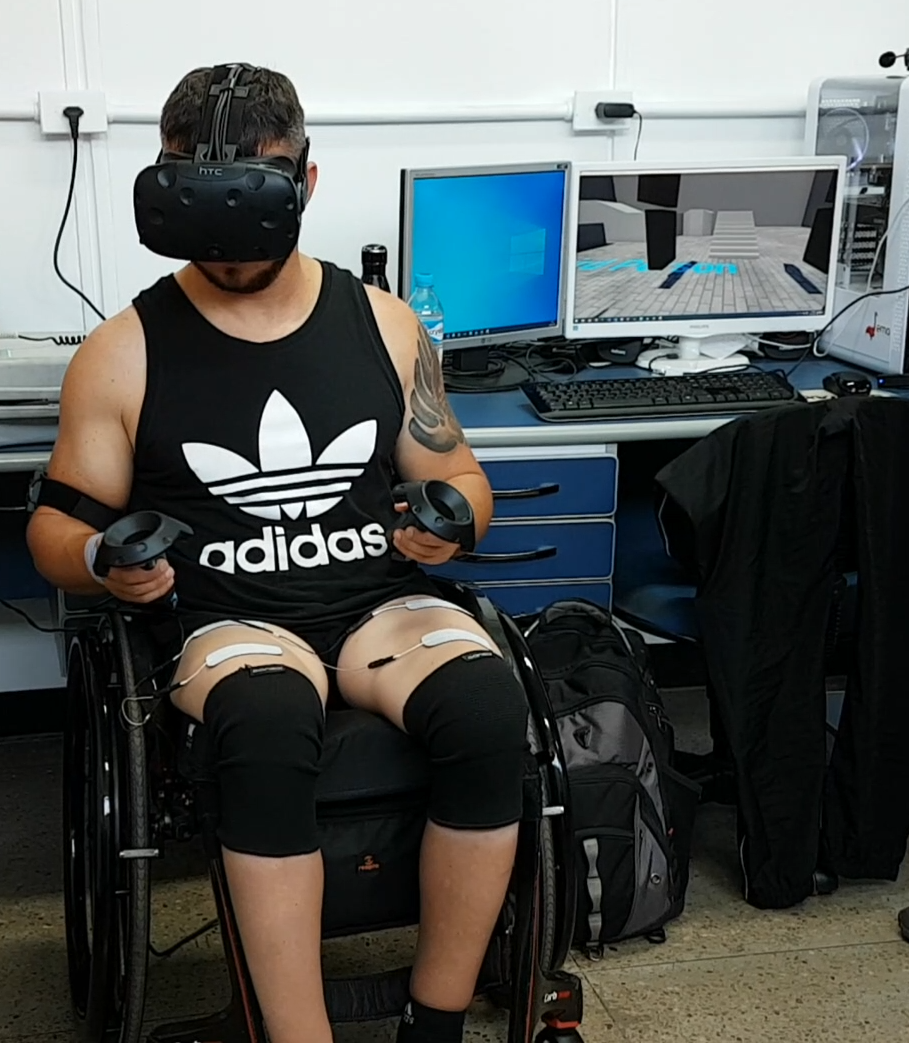
\includegraphics[width=0.55\textwidth]{figuras/vr_sistema_balbino}

	\vspace{4pt}
	{\footnotesize Fonte: \citeonline{balbino2020}. O voluntário utiliza o HMD e os controles do
	HTC Vive e uma IMU no braço direito; a visão do ambiente virtual é espelhada no monitor ao lado.}
\end{figure}

O hardware de imersão empregado é o \emph{HTC Vive} de primeira geração, com rastreamento
externo por estações de base e dois controles de movimento (\emph{Wands}). Um ponto que
merece registro, por corrigir uma imprecisão recorrente, diz respeito ao escopo do movimento
capturado: a análise do repositório e a documentação da fonte mostram que as orientações
provenientes dos sensores inerciais são aplicadas tanto aos \textbf{membros inferiores}
quanto aos \textbf{membros superiores} do avatar. Adicionalmente, os braços podem ser
controlados pelos controles de movimento do HTC Vive por meio de cinemática inversa, e uma
IMU no braço é utilizada para estimar a velocidade de deslocamento nas atividades de marcha.

\section{Arquitetura Atual (As-Is)}
\label{sec:vr-asis}

A arquitetura documentada do sistema, reproduzida na Figura~\ref{fig:vr-arq-doc}, organiza-se
em três blocos: o usuário e os seus sensores; um conjunto de \emph{scripts} em Python; e a
aplicação de realidade virtual construída sobre a \emph{game engine} \emph{Unreal Engine}. As
IMUs capturam o movimento dos membros e um \emph{script} em Python --- que inclui um servidor
responsável pelo cálculo de velocidade --- transmite as orientações à \emph{engine}. Na
\emph{engine}, o avatar tem a sua animação, aparência e câmera controladas por esses dados,
e o ambiente renderizado é exibido no HMD, fechando o laço de realimentação visual com o
usuário.

\begin{figure}[H]
	\centering
	\caption{Arquitetura do sistema de realidade virtual, conforme documentada na fonte.}
	\label{fig:vr-arq-doc}
	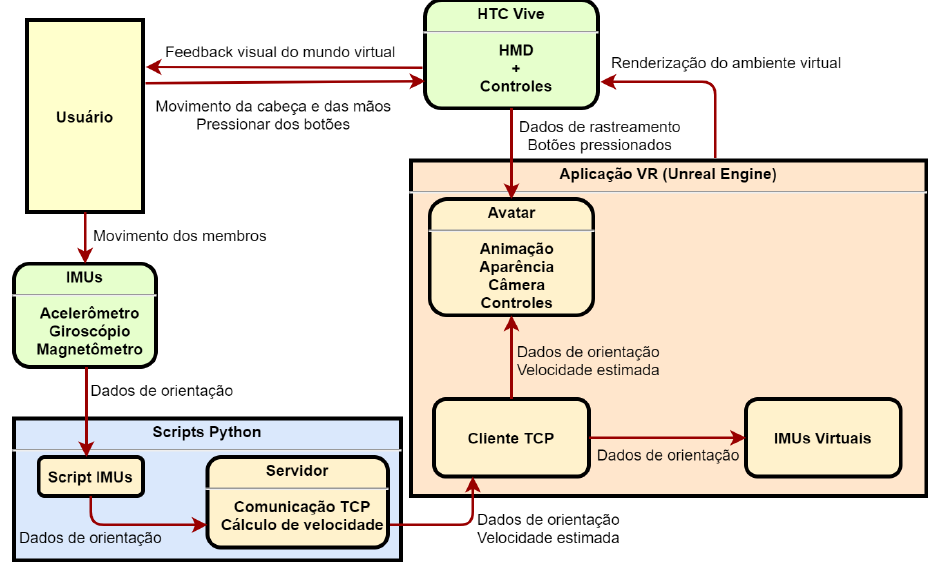
\includegraphics[width=0.95\textwidth]{figuras/vr_arquitetura_balbino}

	\vspace{4pt}
	{\footnotesize Fonte: \citeonline{balbino2020}.}
\end{figure}

A análise do código-fonte confirma o desenho documentado, mas revela camadas adicionais que
a documentação não explicita --- exatamente o tipo de distância entre o \emph{registrado} e o
\emph{montado} que este trabalho investiga. Três observações destacam-se. Primeira, quanto à
\emph{comunicação}: além do canal por \emph{socket} TCP entre o servidor Python e a
\emph{engine} (o mecanismo documentado na Figura~\ref{fig:vr-arq-doc}), o repositório contém
ainda uma integração via \emph{plugin} \emph{ROSIntegration} (uma ponte estilo
\emph{rosbridge}), remanescente de uma abordagem anterior. Coexistem, assim, dois mecanismos
de comunicação no mesmo código, sem que uma camada única e documentada prevaleça. Segunda,
quanto à \emph{localização da lógica}: a aplicação das orientações aos ossos do avatar ---
o núcleo funcional do sistema --- está implementada majoritariamente em \emph{Blueprints}, a
linguagem visual da Unreal Engine. Por serem artefatos binários, os \emph{Blueprints} não
permitem comparação de versões (\emph{diff}) nem revisão de código no mesmo sentido que o
código textual, o que reduz a rastreabilidade e dificulta a manutenção. Terceira, quanto ao
\emph{acoplamento}: o tratamento das orientações e a sua conversão em movimento do avatar
encontram-se embarcados dentro da própria \emph{engine}, de modo que decisões que deveriam
ser independentes --- trocar o capacete, migrar de \emph{engine} ou substituir o sensor ---
repercutem sobre componentes que não deveriam ser afetados, elevando o custo de qualquer
evolução.

\section{Tentativa de Reprodução}
\label{sec:vr-reproducao}

A primeira barreira à reprodução é a \emph{ausência de um \texttt{README}} ou de qualquer
documentação de instalação no repositório --- ausência confirmada por inspeção direta,
diferentemente de outros repositórios do laboratório que dispõem de documentação (ver
Capítulo~\ref{cap:diagnostico}). Não há indicação da versão da \emph{engine}, das
dependências, dos passos de configuração do ambiente nem do procedimento para executar o
sistema. A reconstrução do funcionamento depende, assim, de engenharia reversa a partir do
código e do histórico de \emph{commits}, agravada pelo fato de parte substancial da lógica
residir em \emph{Blueprints} binários. Some-se a isso a dependência de uma geração de
hardware de RV descontinuada (o HTC Vive de primeira geração) e a necessidade de verificar a
integridade dos modelos e \emph{assets} do avatar --- itens cuja disponibilidade só pode ser
plenamente confirmada na estação de trabalho do laboratório, etapa reservada à continuidade
do trabalho.

\section{Limitações Específicas Identificadas}
\label{sec:vr-limitacoes}

Consolidam-se, a seguir, as limitações específicas deste estudo de caso, sem prejuízo das
limitações comuns tratadas no Capítulo~\ref{cap:diagnostico}:

\begin{itemize}
	\item \textbf{Ausência de documentação de instalação e uso:} inexistência de
	      \texttt{README}, de guia de dependências e de passo a passo de execução.
	\item \textbf{Lógica central em artefatos binários:} dependência de \emph{Blueprints}
	      para a lógica de aplicação do movimento, o que compromete a rastreabilidade, a
	      revisão e a comparação de versões.
	\item \textbf{Arquitetura monolítica e acoplada:} lógica de aquisição entrelaçada à
	      lógica de interface dentro da \emph{engine}, dificultando a substituição de
	      componentes.
	\item \textbf{Camada de comunicação não unificada:} coexistência de uma ponte via
	      ROSIntegration e de comunicação por \emph{socket} TCP, sem uma camada única e
	      documentada.
	\item \textbf{Dependência de tecnologia descontinuada:} sistema construído sobre uma
	      geração de hardware de RV (HTC Vive de primeira geração) já descontinuada.
	\item \textbf{Risco quanto aos \emph{assets}:} necessidade de verificar a
	      disponibilidade e a integridade dos modelos e recursos gráficos do avatar
	      (\emph{a confirmar na reprodução}).
\end{itemize}
